\documentclass[12pt]{article}
\usepackage[utf8]{inputenc}
\usepackage{float}
\usepackage{amsmath}


\usepackage[hmargin=3cm,vmargin=6.0cm]{geometry}
%\topmargin=0cm
\topmargin=-2cm
\addtolength{\textheight}{6.5cm}
\addtolength{\textwidth}{2.0cm}
%\setlength{\leftmargin}{-5cm}
\setlength{\oddsidemargin}{0.0cm}
\setlength{\evensidemargin}{0.0cm}

%misc libraries goes here
\usepackage{tikz}
\usetikzlibrary{automata,positioning}

\begin{document}

\section*{Student Information } 
%Write your full name and id number between the colon and newline
%Put one empty space character after colon and before newline
Full Name : Mert Akça  \\
Id Number : 2171163 \\

% Write your answers below the section tags
\section*{Answer 1}

\subsection*{a.}


\begin{table}[h]
\centering
\caption{Rational Numbers}
\label{my-label}
\begin{tabular}{llllll}
  & 1   & 2   & 3   & 4   & 5   \\
1 & 1/1 & 1/2 & 1/3 & 1/4 & 1/5 \\
2 & 2/1 & 2/2 & 2/3 & 2/4 & 2/5 \\
3 & 3/1 & 3/2 & 3/3 & 3/4 & 3/5 \\
4 & 4/1 & 4/2 & 4/3 & 4/4 & 4/5 \\
5 & 5/1 & 5/2 & 5/3 & 5/4 & 5/5
\end{tabular}
\end{table}

We can write set of rational numbers between (0,1) R = {1/2, 1/3, 2/3, 1/4, 1/5, 3/4, 2/5...}. Because there is one-to-one correspondence between the elements of the set R and the set of natural numbers, set of rational numbers countable and infinite. If we multiply all the members with -1, we obtain the set of rational numbers in (-1, 0) which is also countable and infinite.

\subsection*{b.}

\subsection*{c.}

\section*{Answer 2}

\subsection*{a.}

\begin{tikzpicture}[ shorten >=1pt , node distance =4cm , on grid , auto ]
\node [ state , initial, accepting ] (q_0) {$q_0$};
\node [ state, accepting ] (q_1) [ above right = of q_0] {$q_1$};
\node [ state, accepting ] (q_2) [ below right = of q_0] {$q_2$};
\node [ state , accepting ](q_3) [ right = of q_1] {$q_3$};
\node [state] (q_4) [right = of q_2] {$q_4$};
\path [->]
(q_0) edge node {a} (q_1)
edge node [ swap ] {b} (q_2)
(q_1) edge node {b} (q_3)
edge [ loop above ] node {a} ()
(q_2) edge node [ swap ] {a} (q_4)
edge [ loop below ] node {b} ()
(q_3) edge node [swap] {a,b} (q_4)
(q_4) edge [loop below] node {a,b} ();
\end{tikzpicture}

\subsection*{b.}

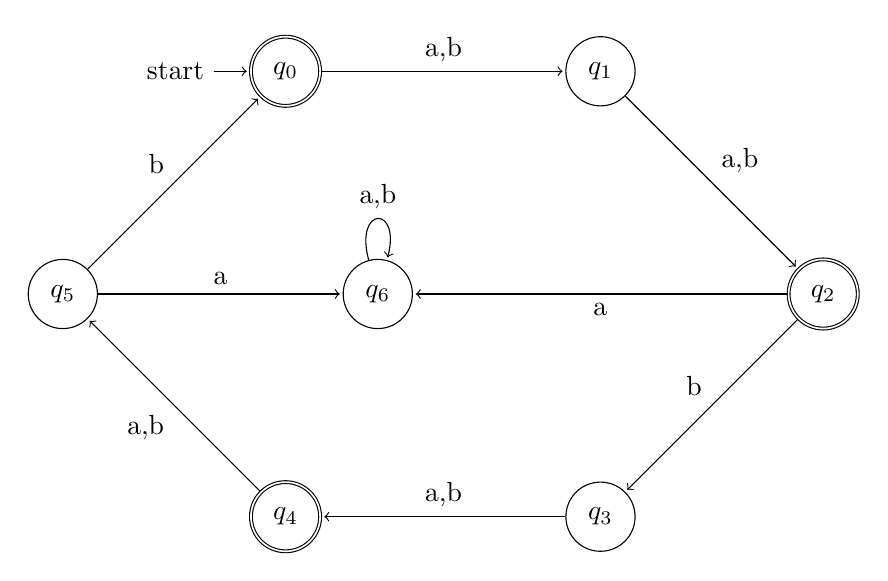
\begin{tikzpicture}[ shorten >=1pt , node distance =4cm , on grid , auto ]
\node [ state , initial, accepting ] (q_0) {$q_0$};
\node [ state ] (q_1) [right = of q_0] {$q_1$};
\node [ state, accepting ] (q_2) [ below right = of q_1] {$q_2$};
\node [ state ](q_3) [ below left = of q_2] {$q_3$};
\node [state, accepting] (q_4) [left = of q_3] {$q_4$};
\node [ state ](q_5) [ below left = of q_0] {$q_5$};
\node [state](q_6) [right = of q_5] {$q_6$};
\path [->]
(q_0) edge node {a,b} (q_1)
(q_1) edge node {a,b} (q_2)
(q_2) edge node [swap] {b} (q_3)
 edge node {a} (q_6)
(q_3) edge node [swap] {a,b} (q_4)
(q_4) edge node {a,b} (q_5)
(q_5) edge node {b} (q_0)
edge node {a} (q_6)
(q_6) edge [loop above] node {a,b} ();
\end{tikzpicture}

\subsection*{c.}

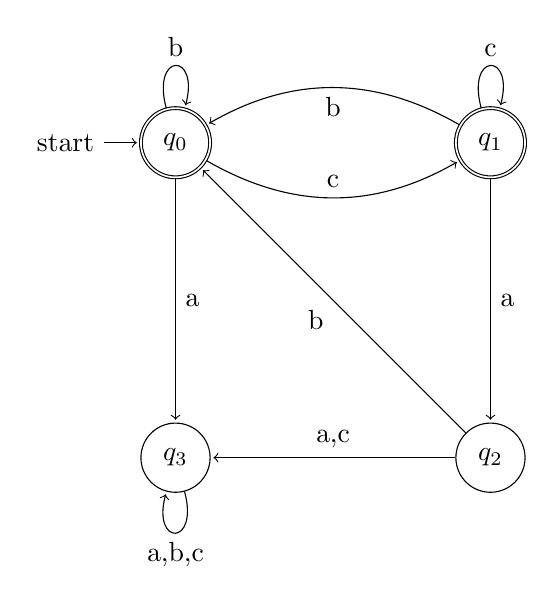
\begin{tikzpicture}[ shorten >=1pt , node distance =4cm , on grid , auto ]
\node [ state , initial, accepting ] (q_0) {$q_0$};
\node [ state, accepting ] (q_1) [ right = of q_0] {$q_1$};
\node [ state ] (q_2) [ below  = of q_1] {$q_2$};
\node [ state  ](q_3) [ below = of q_0] {$q_3$};
\path [->]
(q_0) edge [bend right]  node  {c} (q_1)
edge node {a} (q_3)
edge [loop above] node {b} ()
(q_1) edge [bend right] node {b} (q_0)
edge [ loop above ] node {c} ()
edge node {a} (q_2)
(q_2) edge node [ swap ] {a,c} (q_3)
edge  node {b} (q_0)
(q_3) edge [loop below] node {a,b,c} ();
\end{tikzpicture}



\section*{Answer 3}


\subsection*{a.}
$w_1$ is not in L(N)

\subsection*{b.}
$w_2$ is in L(N)




\section*{Answer 4}

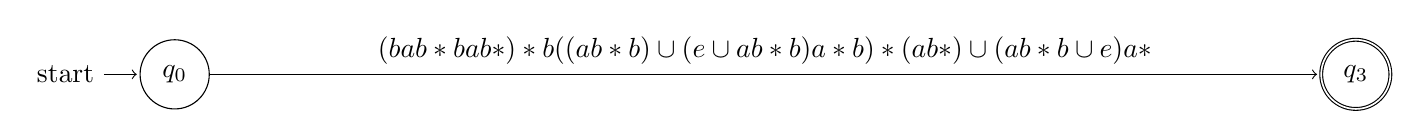
\begin{tikzpicture}[ shorten >=1pt , node distance =15cm , on grid , auto ]
\node [ state , initial ] (q_0) {$q_0$};
\node [ state, accepting ] (q_3) [ right = of q_0] {$q_3$};
\path [->]
(q_0) edge node {$(bab*bab*)*b((ab*b)\cup (e \cup ab*b)a*b)*(ab*) \cup (ab*b \cup e)a*$} (q_3);
\end{tikzpicture}



\section*{Answer 5}

\subsection*{a.}

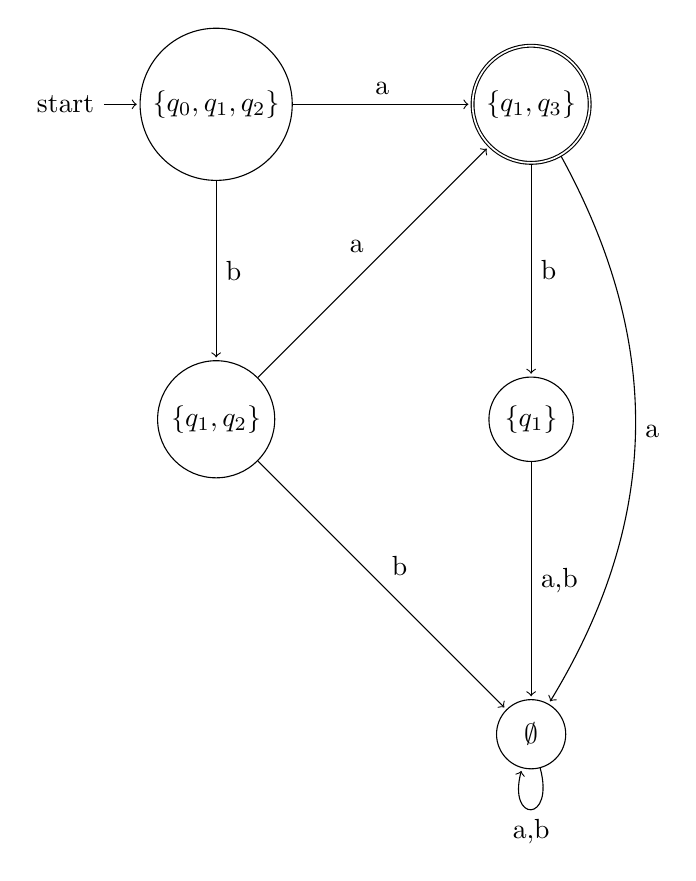
\begin{tikzpicture}[ shorten >=1pt , node distance =4cm , on grid , auto ]
\node [ state , initial ] (q_0) {$\{q_0, q_1, q_2\}$};
\node [ state, accepting ] (q_1) [ right = of q_0] {$\{q_1, q_3\}$};
\node [ state ] (q_2) [ below  = of q_0] {$\{q_1, q_2\}$};
\node [ state  ](q_3) [ below = of q_1] {$\{q_1\}$};
\node [ state  ](q_4) [ below = of q_3] {$\emptyset$};
\path [->]
(q_0) edge node {a} (q_1)
edge node {b} (q_2)
(q_1) edge node {b} (q_3)
edge [bend left] node {a} (q_4)
(q_2) edge node {a} (q_1)
edge  node {b} (q_4)
(q_3) edge node {a,b} (q_4)
(q_4) edge [loop below] node {a,b} ();
\end{tikzpicture}

\subsection*{b.}

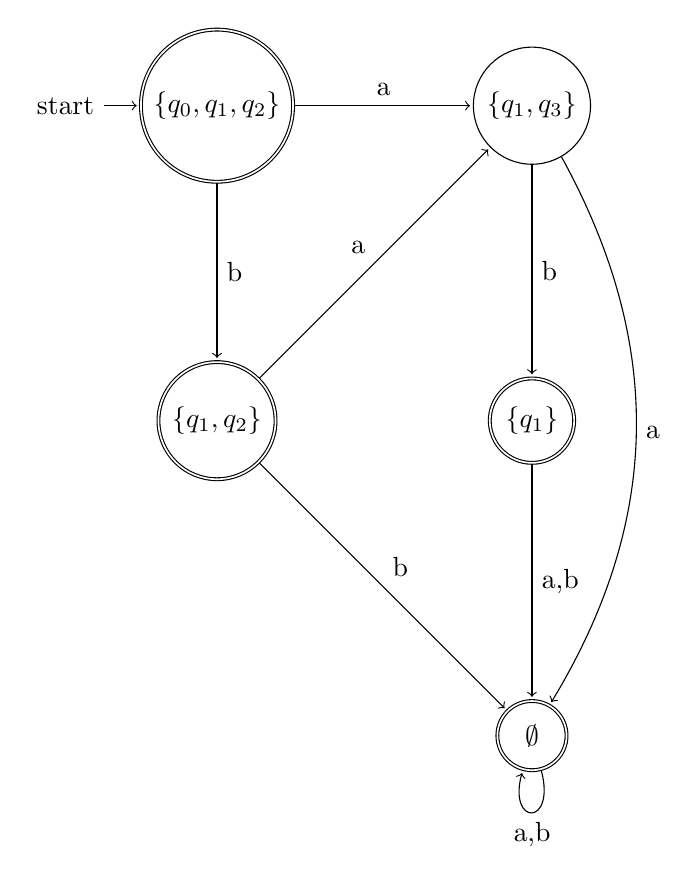
\begin{tikzpicture}[ shorten >=1pt , node distance =4cm , on grid , auto ]
\node [ state , initial, accepting ] (q_0) {$\{q_0, q_1, q_2\}$};
\node [ state] (q_1) [ right = of q_0] {$\{q_1, q_3\}$};
\node [ state, accepting ] (q_2) [ below  = of q_0] {$\{q_1, q_2\}$};
\node [ state , accepting  ](q_3) [ below = of q_1] {$\{q_1\}$};
\node [ state , accepting  ](q_4) [ below = of q_3] {$\emptyset$};
\path [->]
(q_0) edge node {a} (q_1)
edge node {b} (q_2)
(q_1) edge node {b} (q_3)
edge [bend left] node {a} (q_4)
(q_2) edge node {a} (q_1)
edge  node {b} (q_4)
(q_3) edge node {a,b} (q_4)
(q_4) edge [loop below] node {a,b} ();
\end{tikzpicture}



\section*{Answer 6}




\section*{Answer 7}

\subsection*{a.}

Let $w = aabbaa$, which the number of a's is 4.


\noindent If we choose $x=aa$, $y=bba$, $z=a$, it becomes,  $xy^iz=aa(bba)^ia$

\noindent Let $i=2$, $xy^2z = aabbabbaa$, the number of a's is 5 which does not meet the rule. Furthermore, the language cannot be a regular language

\end{document}

​


